\documentclass[12pt]{article}
\usepackage[margin=1in]{geometry}
\usepackage[utf8]{inputenc}
\usepackage{hyperref}
\usepackage{graphicx}
\usepackage{listings}
\usepackage{xcolor}
\usepackage{datetime}
\usepackage{framed}
\usepackage{float}
\usepackage{forest}

\graphicspath{
    {images/}
}

\hypersetup{
    colorlinks=true,
    linkcolor=black,
    filecolor=magenta,      
    urlcolor=blue,
    citecolor=blue
}

% Both single quotes
\def\bsq#1{\lq{#1}\rq}

\definecolor{codegreen}{rgb}{0,0.6,0}
\definecolor{codegray}{rgb}{0.5,0.5,0.5}
\definecolor{codepurple}{rgb}{0.58,0,0.82}

\lstdefinestyle{mystyle}{
    basicstyle=\ttfamily\footnotesize,
    commentstyle=\color{codegreen},
    keywordstyle=\color{magenta},
    stringstyle=\color{codepurple},
    keywordstyle=[2]\color{blue},
    breakatwhitespace=false,         
    breaklines=true,                 
    captionpos=b,                    
    keepspaces=true,                 
    numbers=left,                    
    numbersep=5pt,                  
    showspaces=false,                
    showstringspaces=false,
    showtabs=false,                  
    tabsize=2
}

\lstset{
    style=mystyle,
    frame=single,
    numbers=none,
    upquote=true
}

\title{Airplane Boarding}
\author{Steven Yulong Yan}

\begin{document}

\newdate{date}{20}{11}{2020}
\date{\displaydate{date}}

\maketitle

\tableofcontents

\newpage

\section{Introduction}
What is the best way to board an airplane? 
\\[0.1in]
Modern airlines adopt three main approaches when it comes to boarding passengers:
the front-row-first method, the back-row-first method and the window-to-middle method.
This report compares the time complexity of those three methods and determines the fastest
way among them using a Python program.

\section{Model}

\begin{enumerate}
    \item Back-row-first boarding: The back-row-first boarding can be interpreted as
    pouring people into the airplane back to front. In a back-row-first boarding,
    the process is smooth while the first boarding group are walking to the back of the plane.
    But when the first person stops and starts to unload their luggage the second person
    cannot get to their seat even if their seat is in view. This causes the entire
    queue to halt until the first person gets out of the way and the queue resumes.
    This approach is very similar to how we would do when we are filling a cylinder.
    This is a sensible solution which is also easy to implement. However,
    the back-row-first boarding method can be very ineffective due to process described above amounting to aggregate
    loss of time from those boarding the plane when one person stops and stows their bag.
    \item Front-row-first boarding: The front-row-first method is essentially the reverse order of the
    back-row-first approach. This approach is inefficient as it causes the vast majority of the passengers to wait
    outside of the airplane for a longer amount of time.
    \item Window-to-middle boarding: The window-to-middle method fills up the seats of
    a plane one column at a time, starting from the column closest to the window and
    moving towards the column next to the aisle. This approach is able to eliminate
    some sources of boarding delay such as bag stowage and seat shuffles.
\end{enumerate}

\section{Implementation}

\begin{enumerate}
    \item Import from libraries (plotting, multithreading, tabling).
    \item Make the assumption of time spent on certain activities (the average time for getting seated, the standard deviation time for getting seated, minimum possible boarding time, time needed to walk to the next row).
    \item Create the Passenger, Plane, Boarding classes and their methods.
    \item Define the three different boarding methods and use the table output to verify the order in which the passengers are seated and that the methods are implemented correctly.
    \item Use threading to simulate the time elapsed during boarding on a plane with 800 seats (Running the program will take a while).
\end{enumerate}




\newpage

\section{Codebase}

\begin{lstlisting}[language=python]
from matplotlib.pyplot import *
from multiprocessing.pool import ThreadPool
from tabulate import *

T_AVG_SEATING = 6
T_STDDEV_SEATING = 4
T_MIN_BOARDING = 2
T_TO_NEXT = 1


class Passenger:
    def __init__(self, row_num, seat_num, pos=None):
        self.id = None
        self.row_num = row_num
        self.seat_num = seat_num
        self.position = pos
        self.boarded = False
        self.boarding_status = "waiting"
        self.time_until_seated = None
        self.waiting_time = 0

    def set_id(self, passenger_id):
        self.id = passenger_id

    def set_position(self, position):
        self.position = position

    def set_time_until_seated(self, time_until_seated):
        self.time_until_seated = time_until_seated

    def set_boarding_status(self, boarding_status):
        self.boarding_status = boarding_status

    def include_waiting_time(self, t):
        self.waiting_time += t


class Plane:
    def __init__(self, row_num, seat_num_per_row):
        self.row_num = row_num
        self.occupied_rows = {rowNum: False for rowNum in range(row_num)}
        self.seat_num_per_row = seat_num_per_row
        self.passenger_total_num = row_num * seat_num_per_row
        self.passenger_boarded_num = 0
        self.passengers = None

    def generate_passengers(self, method):
        unordered_passengers = [
            Passenger(rowNumber, seatNumber)
            for rowNumber in range(self.row_num)
            for seatNumber in range(self.seat_num_per_row)
        ]
        passengers_ordered = front_row_first(unordered_passengers)
        if method == "back-row-first":
            passengers_ordered = back_row_first(unordered_passengers)
        elif method == "window-to-middle":
            passengers_ordered = window_to_middle(unordered_passengers)

        for n, passenger in enumerate(passengers_ordered):
            passenger.set_id(n)
            passenger.set_position(-1 * n - 1)

        return passengers_ordered

    def board(self, boarding_method):
        self.passenger_boarded_num = 0
        self.passengers = self.generate_passengers(boarding_method)
        self.move_passengers()
        return max(list(map(lambda x: x.waiting_time, self.passengers))) / 60

    def set_boarding_status(self, passenger, boarding_status):
        passenger.set_boarding_status(boarding_status)

        if boarding_status == "seated":
            self.passenger_boarded_num += 1
            assert (passenger.position == passenger.row_num)
            self.occupied_rows[passenger.position] = False
        elif boarding_status == "seating":
            self.occupied_rows[passenger.position] = True

    def move_passengers(self):
        while self.passenger_boarded_num < self.passenger_total_num:
            for passenger in self.passengers:
                if passenger.boarding_status == "seating":
                    passenger.set_time_until_seated(
                        passenger.time_until_seated - 1
                    )
                    passenger.include_waiting_time(T_TO_NEXT)
                    if passenger.time_until_seated <= 0:
                        self.set_boarding_status(passenger, "seated")
                elif passenger.boarding_status == "waiting":
                    if passenger.position < passenger.row_num and \
                            self.occupied_rows[passenger.position + 1] is False:
                        self.occupied_rows[passenger.position] = False
                        passenger.set_position(passenger.position + 1)
                        self.occupied_rows[passenger.position] = True
                        passenger.include_waiting_time(T_TO_NEXT)
                        if passenger.position == passenger.row_num:
                            self.set_boarding_status(passenger, "seating")
                            seating_time = max(np.random.normal(
                                T_AVG_SEATING,
                                T_STDDEV_SEATING,
                                1)[0], T_MIN_BOARDING)
                            passenger.set_time_until_seated(seating_time)
                    elif self.occupied_rows[passenger.position + 1]:
                        passenger.include_waiting_time(T_TO_NEXT)
                elif passenger.boarding_status == "seated":
                    continue


class Boarding:
    def __init__(self, target_plane):
        self.target_plane = target_plane
        self.passenger_num = target_plane["row_num"] * \
            target_plane["seat_num_per_row"]

    def boarding_plane(self, policy):
        return Plane(**self.target_plane).board(policy)

    def boarding_thread(self, method, n=100):
        pool = ThreadPool(16)
        output = pool.map(self.boarding_plane, [method] * n)
        pool.close()
        pool.join()
        return output

    def plot(self, input_methods, iter_per_method=100):
        figure()
        title("Calculated Boarding Time from Different Approaches")
        ylabel("Count")
        xlabel("Boarding Time (min)")
        colors = ["red", "blue", "green"]

        for n, method in enumerate(input_methods):
            color = colors[n]
            times = self.boarding_thread(method, n=iter_per_method)
            _ = hist(times, color=color, alpha=0.9)
            axvline(np.mean(times), c=color, label="{}".format(method))
            legend()

        show()


def front_row_first(target_passengers):
    return sorted(target_passengers,
                  key=lambda passenger: passenger.row_num)


def back_row_first(target_passengers):
    return sorted(target_passengers,
                  key=lambda passenger: -1 * passenger.row_num)


def window_to_middle(target_passengers):
    return sorted(target_passengers,
                  key=lambda passenger:
                  (passenger.seat_num, -1 * passenger.row_num))


def main():
    methods = ["front-row-first", "back-row-first", "window-to-middle"]

    for i in methods:
        print("For {}:".format(i))
        plane = Plane(row_num=10, seat_num_per_row=4)
        passengers = plane.generate_passengers(i)
        results = [(x.row_num + 1, x.seat_num + 1) for x in passengers]
        print(tabulate(results, headers=["Row", "Seat"]))
        print()

    Boarding({"row_num": 100, "seat_num_per_row": 8}) \
        .plot(methods, iter_per_method=100)


if __name__ == '__main__':
    main()
\end{lstlisting}

\begin{framed}
    \fontsize{9}{9}\selectfont
    \begin{verbatim}
For front-row-first:
  Row    Seat
-----  ------
    1       1
    1       2
    1       3
    1       4
    2       1
    2       2
    2       3
    2       4
    3       1
    3       2
    3       3
    3       4
    4       1
    4       2
    4       3
    4       4
    5       1
    5       2
    5       3
    5       4
    6       1
    6       2
    6       3
    6       4
    7       1
    7       2
    7       3
    7       4
    8       1
    8       2
    8       3
    8       4
    9       1
    9       2
    9       3
    9       4
   10       1
   10       2
   10       3
   10       4

For back-row-first:
  Row    Seat
-----  ------
   10       1
   10       2
   10       3
   10       4
    9       1
    9       2
    9       3
    9       4
    8       1
    8       2
    8       3
    8       4
    7       1
    7       2
    7       3
    7       4
    6       1
    6       2
    6       3
    6       4
    5       1
    5       2
    5       3
    5       4
    4       1
    4       2
    4       3
    4       4
    3       1
    3       2
    3       3
    3       4
    2       1
    2       2
    2       3
    2       4
    1       1
    1       2
    1       3
    1       4

For window-to-middle:
  Row    Seat
-----  ------
   10       1
    9       1
    8       1
    7       1
    6       1
    5       1
    4       1
    3       1
    2       1
    1       1
   10       2
    9       2
    8       2
    7       2
    6       2
    5       2
    4       2
    3       2
    2       2
    1       2
   10       3
    9       3
    8       3
    7       3
    6       3
    5       3
    4       3
    3       3
    2       3
    1       3
   10       4
    9       4
    8       4
    7       4
    6       4
    5       4
    4       4
    3       4
    2       4
    1       4
    \end{verbatim}
\end{framed}

\begin{figure}[H]
    \centering
    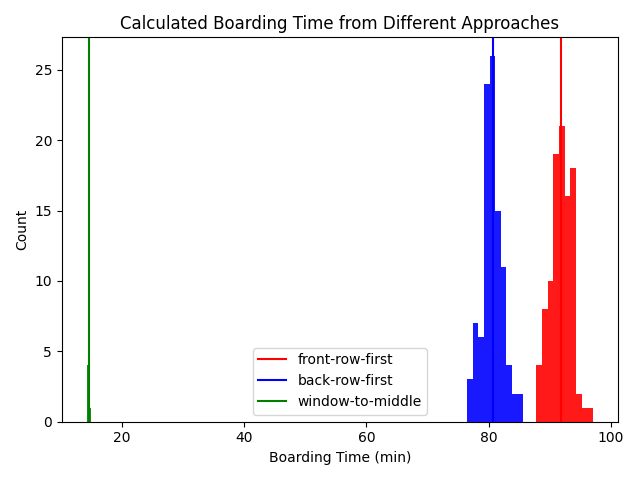
\includegraphics[width=1\textwidth]{1.png}
\end{figure}


\newpage

\section{Conclusion}

The window-to-middle boarding method is a smart boarding strategy that
maximises parallel boarding, therefore minimising the time bottlenecks occurred in
the boarding process. This method is the fastest of the three as it minimises
seat shuffles such that a person does not have to get out of their row for
another person to get into it.

\end{document}
